% Abstracts are usually written in English, with a version in your
% mother tongue underneath
\chapter*{Abstract} 
\addcontentsline{toc}{chapter}{Abstract}

% Don't change anything above this.
The applications of machine learning have created an opportunity to deal with complex problems currently encountered in radio astronomy data processing. Calibration is one of the most important data processing steps required to produce high dynamic range images. This process involves the determination of calibration parameters, both instrumental and astronomical, to correct the
collected data. These parameters include instrumental as well as astronomical parameters. Typically, astronomers use a package such as Common Astronomy Software Applications (CASA) to compute the gain solutions based on regular observations of a known calibrator source. In this work we present applications of machine learning to first generation calibration (1GC), using the KAT-7 telescope environmental and pointing sensor data recorded during observations. Applying machine learning to 1GC, as opposed to calculating the gain solutions in CASA, has shown evidence of reducing computation, as well as accurately predict the 1GC gain solutions and antenna behaviour. These methods are computationally less expensive, however they have not fully learned to generalise  in predicting  accurate 1GC solutions by looking at environmental and pointing sensors. We call this multi-output regression model $\textit{ZCal}$, which is based on random forest, decision trees, extremely randomized trees and K-nearest neighbor algorithms. The prediction error obtained during the testing of our model on testing data is $\approx$ $0.01< \mathrm{rms}_\mathrm{e} <0.09$ for gain amplitude per antenna, and 0.2 $\mathrm{rad}< \mathrm{rms}_\mathrm{e}<$0.5 $\mathrm{rad}$ for gain phase. This shows that the instrumental parameters used to train our model strongly correlate with gain amplitude effects than phase.  
% At a unviersity like Stellenbosch you *must* produce an abstract in Afrikaans for your masters.
% At AIMS you are encouraged to repeat the abstract in your mother tongue
% French, Igbo, Mlagasy, etc. just write it using LaTeX's special
% characters.
% Arabic students see the arabic.tex file for an example
% Amharic use openoffice and export from there and import a figure here.
% Where the words do not exist put the English work in italics, or use mathematical symbols.


% Do not change anything below this except for adding your
% signature (replace images/signature.png) and your name.
\vfill
\newpage
\section*{Declaration}
I, the undersigned, hereby declare that the work contained in this thesis is my original work, and that any work done by others or by myself previously has been acknowledged and referenced accordingly.

% Scan your signature into a small picture called 'signature.png' and insert it
% above your name and the date:
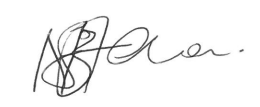
\includegraphics[height=2cm]{images/Signature.png} \newline \hrule
% Your name must be in English Capitalisation with no comma, and the Family name comes last. 
% Do note the date below. It is called the "deadline".
Simphiwe Nhlanhla Zitha,  18 December 2018

